\documentclass[runningheads]{llncs}

\usepackage[utf8]{inputenc}
\usepackage{amsmath}
\usepackage{amsfonts}
\usepackage{amssymb}
\usepackage{graphicx}
\usepackage{algorithm}
\usepackage{algorithmic}
\usepackage{booktabs}
\usepackage{url}
\usepackage[colorlinks=true, citecolor=blue, linkcolor=blue, urlcolor=blue]{hyperref}

\begin{document}

\title{Implementation of Shrinkage Estimators for Cosmological Precision Matrices in TEDA: Enhancing Ensemble-Based Data Assimilation in High-Dimensional Settings\thanks{TEDA source code is available at: \url{https://github.com/enino84/TEDA.git}}}

\titlerunning{Shrinkage Estimators for Cosmological Precision Matrices in TEDA}

\author{Elias D. Nino-Ruiz\inst{1}\orcidID{0000-0001-7420-4517} \and
Andr\'es Movilla Obreg\'on\inst{1}}

\authorrunning{E. D. Nino-Ruiz and A. Movilla Obreg\'on}

\institute{Department of Computer Science and Statistics, Universidad del Norte, Barranquilla, Colombia\\
\email{\{enino, movillaf\}@uninorte.edu.co}}

\maketitle

\begin{abstract}
We implement six shrinkage-based precision matrix estimators in the TEDA educational data assimilation framework: three direct precision shrinkage variants from Looijmans et al.\ (identity, eigenvalue, and cosmological targets), a scaled identity variant we propose as a domain-agnostic alternative, the NERCOME estimator, and Ledoit-Wolf covariance shrinkage. Tests on the Lorenz~96 system ($n=40$) and BOSS DR12 cosmological mock data ($d=18$) show that direct precision shrinkage performance depends on how well the target matches the true precision structure---the methods fail on Lorenz~96 (dense off-diagonal precision) but give the best standalone estimates on near-diagonal cosmological data. We also find that good standalone estimation does not imply good filtering: Ledoit-Wolf produces the worst precision estimates on cosmological data yet the lowest EnKF RMSE, because its low variance pays off when errors compound over repeated assimilation cycles. All code is publicly available in TEDA.

\keywords{Data Assimilation \and Ensemble Kalman Filter \and Shrinkage Estimation \and Cosmological Precision Matrix \and Covariance Matrix Estimation \and TEDA \and Python}
\end{abstract}

\section{Introduction}
\label{sec:introduction}

Ensemble Kalman filters require the inverse of the background error covariance matrix, but in most operational settings the ensemble is far too small to estimate that matrix reliably. When the state dimension $n$ exceeds the ensemble size $N_e$, the sample covariance is rank-deficient and cannot be inverted at all~\cite{houtekamer1998data}; even when $N_e > n$, sampling noise introduces spurious correlations that contaminate the precision matrix~\cite{anderson2001ensemble}. The same problem appears in cosmological data analysis, where the number of mock catalogs available to estimate power spectrum covariances is often comparable to the data dimension~\cite{hamilton2006measuring}.

Shrinkage estimation addresses this by combining the noisy sample estimate with a structured, low-variance target matrix, accepting some bias in exchange for reduced mean squared error~\cite{ledoit2004well}. Most shrinkage work operates in covariance space: Ledoit and Wolf~\cite{ledoit2004well} derived an optimal intensity for shrinking toward a scaled identity, Pope and Szapudi~\cite{pope2008shrinkage} brought this idea to cosmology, and Chen et al.~\cite{chen2010shrinkage} proposed oracle-approximating algorithms that improve on Ledoit-Wolf in high dimensions. Bodnar et al.~\cite{bodnar2016direct} took a different route, shrinking the precision matrix directly rather than first shrinking the covariance and then inverting. Looijmans et al.~\cite{looijmans2024comparison} applied this direct precision framework to cosmological data, comparing several target choices and showing that domain-informed targets outperform generic ones when the true precision is near-diagonal.

Two gaps remain. First, Looijmans et al.\ used these estimators for standalone precision matrix estimation, not inside a sequential filter. It is unclear whether an estimator that performs well in a one-shot setting will also perform well when applied repeatedly across hundreds of assimilation cycles, where errors in the precision estimate feed back through the forecast model. Second, the direct precision targets in the literature are either generic (identity, eigenvalues) or domain-specific (cosmological), with no middle ground for practitioners who lack prior knowledge of the precision structure but want something better than the identity.

We address both gaps. We embed the Bodnar et al.\ direct precision shrinkage framework inside the dual formulation of the Ensemble Kalman Filter, recomputing the shrinkage coefficients at each assimilation cycle. We propose a scaled identity target that uses empirical per-variable variances as a domain-agnostic alternative to the cosmological target. And we test all methods---three targets from Looijmans et al., our scaled variant, NERCOME~\cite{joachimi2017non}, and Ledoit-Wolf---on two systems with opposite precision structure: Lorenz~96~\cite{lorenz1996predictability} ($n = 40$, dense off-diagonal precision) and BOSS DR12 cosmological mock data~\cite{looijmans2024comparison} ($d = 18$, near-diagonal precision). The experiments show that direct precision shrinkage performance depends on how well the target matches the true precision structure, and that the estimator producing the worst standalone precision estimates (Ledoit-Wolf) yields the best EnKF filtering error, because its low variance pays off over repeated assimilation cycles. All implementations are publicly available in the TEDA framework~\cite{nino2022teda}.

\section{Background and Theory}
\label{sec:background}

\subsection{Ensemble-Based Data Assimilation}
\label{sec:enkf}

The Ensemble Kalman Filter (EnKF)~\cite{evensen2003ensemble} represents the state of a dynamical system using an ensemble of $N_e$ state vectors $\{\mathbf{x}_i^b\}_{i=1}^{N_e}$, each $\mathbf{x}_i^b \in \mathbb{R}^{n \times 1}$. The ensemble mean
\begin{equation}
\bar{\mathbf{x}}^b = \frac{1}{N_e} \sum_{i=1}^{N_e} \mathbf{x}_i^b \in \mathbb{R}^{n \times 1},
\end{equation}
serves as the background state estimate. The background error covariance is estimated from ensemble perturbations. With the deviation matrix
\begin{equation}
\label{eq:deviation}
\Delta\mathbf{X}^b = \mathbf{X}^b - \bar{\mathbf{x}}^b \mathbf{1}^T \in \mathbb{R}^{n \times N_e},
\end{equation}
where $\mathbf{X}^b = [\mathbf{x}_1^b, \ldots, \mathbf{x}_{N_e}^b]$, the sample covariance is
\begin{equation}
\label{eq:sample_cov}
\mathbf{P}^b = \frac{1}{N_e - 1} \Delta\mathbf{X}^b (\Delta\mathbf{X}^b)^T \in \mathbb{R}^{n \times n}.
\end{equation}

Given observations $\mathbf{y} \in \mathbb{R}^{m \times 1}$, the stochastic EnKF computes analysis updates by solving
\begin{equation}
\label{eq:stochastic_enkf}
[\mathbf{H}\mathbf{P}^b\mathbf{H}^T + \mathbf{R}] \, \Delta\mathbf{X}^a = \mathbf{D}^s \in \mathbb{R}^{m \times N_e},
\end{equation}
where $\mathbf{H} \in \mathbb{R}^{m \times n}$ is the observation operator, $\mathbf{R} \in \mathbb{R}^{m \times m}$ the observation error covariance, and $\mathbf{D}^s$ the innovation matrix of perturbed observation departures.

The dual EnKF~\cite{nino2018ensemble} reformulates this in terms of the precision matrix:
\begin{equation}
\label{eq:dual_enkf}
[(\mathbf{P}^b)^{-1} + \mathbf{H}^T\mathbf{R}^{-1}\mathbf{H}] \, \Delta\mathbf{X}^a = \mathbf{H}^T\mathbf{R}^{-1}\mathbf{D}^s \in \mathbb{R}^{n \times N_e}.
\end{equation}
This formulation requires the precision matrix $(\mathbf{P}^b)^{-1}$---the central object of this work. When $N_e < n$, the sample covariance~\eqref{eq:sample_cov} has rank at most $N_e - 1$ and cannot be inverted. Even when $N_e > n$, the sample precision can be poorly conditioned, amplifying noise in the analysis.

A third variant projects the analysis onto the ensemble subspace~\cite{nino2022teda}:
\begin{equation}
\label{eq:ensemble_space}
\mathbf{X}^a = \mathbf{X}^b + \Delta\mathbf{X}^b \mathbf{W}^*,
\end{equation}
where $\mathbf{W}^* \in \mathbb{R}^{N_e \times N_e}$ is obtained from a reduced system, bringing the problem from $n$ dimensions down to $N_e$.

\subsection{Shrinkage Estimation}
\label{sec:shrinkage}

The idea behind shrinkage is to blend the sample covariance with a structured target $\mathbf{T}$:
\begin{equation}
\label{eq:shrinkage_cov}
\hat{\mathbf{P}} = (1 - \lambda) \mathbf{S} + \lambda \mathbf{T},
\end{equation}
where $\lambda \in [0,1]$ controls how much weight goes to the target. At $\lambda = 0$ we recover the sample covariance; at $\lambda = 1$ we use only the target. The optimal $\lambda$ minimizes
\begin{equation}
\label{eq:optimal_lambda}
\lambda^* = \arg\min_{\lambda \in [0,1]} \mathbb{E}\left[\|\hat{\mathbf{P}} - \boldsymbol{\Sigma}\|_F^2\right],
\end{equation}
with $\boldsymbol{\Sigma}$ the true covariance.

\textbf{Ledoit-Wolf estimator.} Ledoit and Wolf~\cite{ledoit2004well} derived a closed-form optimal intensity for the target $\mathbf{T} = \mu \mathbf{I}$, $\mu = \text{tr}(\mathbf{S})/n$:
\begin{equation}
\label{eq:lw_lambda}
\lambda^*_{\text{LW}} = \frac{\sum_{i=1}^{N_e} \|\mathbf{z}_i \mathbf{z}_i^T - \mathbf{S}\|_F^2 / N_e^2}{\|\mathbf{S} - \mu\mathbf{I}\|_F^2},
\end{equation}
where $\mathbf{z}_i$ are standardized observations. This estimator is asymptotically optimal and has become a standard reference in high-dimensional settings.

\textbf{Oracle estimator.} When the true covariance $\boldsymbol{\Sigma}$ is known (as in simulation studies), the oracle intensity
\begin{equation}
\label{eq:oracle}
\lambda^*_{\text{oracle}} = \frac{\text{tr}[(\mathbf{S} - \boldsymbol{\Sigma})(\mathbf{T} - \boldsymbol{\Sigma})]}{\|\mathbf{T} - \mathbf{S}\|_F^2}
\end{equation}
gives a best-case benchmark, useful for judging how close a data-driven estimator gets to the theoretical optimum.

\textbf{Nercome estimator.} NERCOME~\cite{joachimi2017non} is a nonlinear covariance estimator that sidesteps the choice of target entirely. It randomly splits the ensemble into two disjoint subsets, diagonalizes one subset's sample covariance via eigendecomposition, and rotates the other subset's covariance into that eigenbasis, keeping only the diagonal. By averaging over many such random splits and selecting the split ratio that minimizes cross-validated loss, NERCOME produces a better-conditioned estimate without requiring structural assumptions about the covariance.

\subsection{Cosmological Covariance Matrix Structure}
\label{sec:cosmo_cov}

In galaxy surveys, the data vector consists of power spectrum measurements $\hat{C}_\ell$ at different multipole moments $\ell$ and, for tomographic analyses, different redshift bins $z$. For a Gaussian random field observed over a sky fraction $f_{\text{sky}}$, the covariance of power spectrum estimates is~\cite{pope2008shrinkage}:
\begin{equation}
\label{eq:cosmo_cov}
\text{Cov}(\hat{C}_{\ell_i}, \hat{C}_{\ell_j}) = \frac{2}{(2\ell_i + 1) f_{\text{sky}}} \left(C_{\ell_i} + \frac{1}{n_g}\right)^2 \delta_{\ell_i \ell_j},
\end{equation}
where $C_{\ell}$ is the true power spectrum, $n_g$ the galaxy number density, and $\delta_{\ell_i \ell_j}$ the Kronecker delta. The $1/n_g$ term is shot noise, and $(2\ell+1)f_{\text{sky}}$ counts the independent modes $N_\ell$ at multipole $\ell$. The diagonal structure follows from mode independence under the Gaussian assumption.

The precision matrix is then
\begin{equation}
\label{eq:cosmo_precision}
\mathbf{P}_{ij}^{-1} = \frac{(2\ell_i + 1)}{2} f_{\text{sky}} \left(C_{\ell_i} + \frac{1}{n_g}\right)^{-2} \delta_{\ell_i \ell_j} \, \delta_{z_i z_j}.
\end{equation}

This diagonal structure motivates a cosmological shrinkage target. Following Pope and Szapudi~\cite{pope2008shrinkage}, as adopted by Looijmans et al.~\cite{looijmans2024comparison}, the target is
\begin{equation}
\label{eq:cosmo_target}
T^{(2)}_{ii} = \frac{2}{N_{\ell_i}} C_{\ell_i}^2,
\end{equation}
where $N_{\ell_i} = (2\ell_i + 1) f_{\text{sky}}$. This captures the leading-order cosmic variance contribution and, when the assumed power spectrum is close to the truth, provides a much more informative shrinkage direction than a generic identity target.

\subsection{Related Work}
\label{sec:related}

Pope and Szapudi~\cite{pope2008shrinkage} introduced shrinkage estimation to cosmology, showing that even a simple diagonal target improves power spectrum covariance estimation over the raw sample covariance when few simulations are available. Looijmans et al.~\cite{looijmans2024comparison} compared covariance shrinkage (with empirical and analytical targets) against precision shrinkage (with eigenvalue-based and cosmological targets, following Bodnar et al.~\cite{bodnar2016direct}) and the NERCOME estimator. They found that incorporating cosmological prior information helps, especially at larger sample sizes, with the benefit depending on $N_e / n$ and the accuracy of the assumed cosmological model.

Haff~\cite{haff1991variational} derived improved Bayes estimators for the covariance matrix via eigenvalue shrinkage, and Chen et al.~\cite{chen2010shrinkage} proposed oracle-approximating algorithms that improve on Ledoit-Wolf in high dimensions. All of these methods trade bias for variance reduction; they differ in how the target encodes prior assumptions about the covariance structure.

\section{Implementation in TEDA}
\label{sec:methods}

We integrated six shrinkage-based precision matrix estimators into the TEDA framework. Below we describe the software architecture, the algorithms, and the design choices involved.

\subsection{TEDA Architecture Overview}
\label{sec:architecture}

TEDA uses an object-oriented design where dynamical models, ensemble management, observation handling, and analysis methods are separate modular classes. Figure~\ref{fig:class_diagram} shows the relevant class hierarchy.

\begin{figure}[t]
\centering
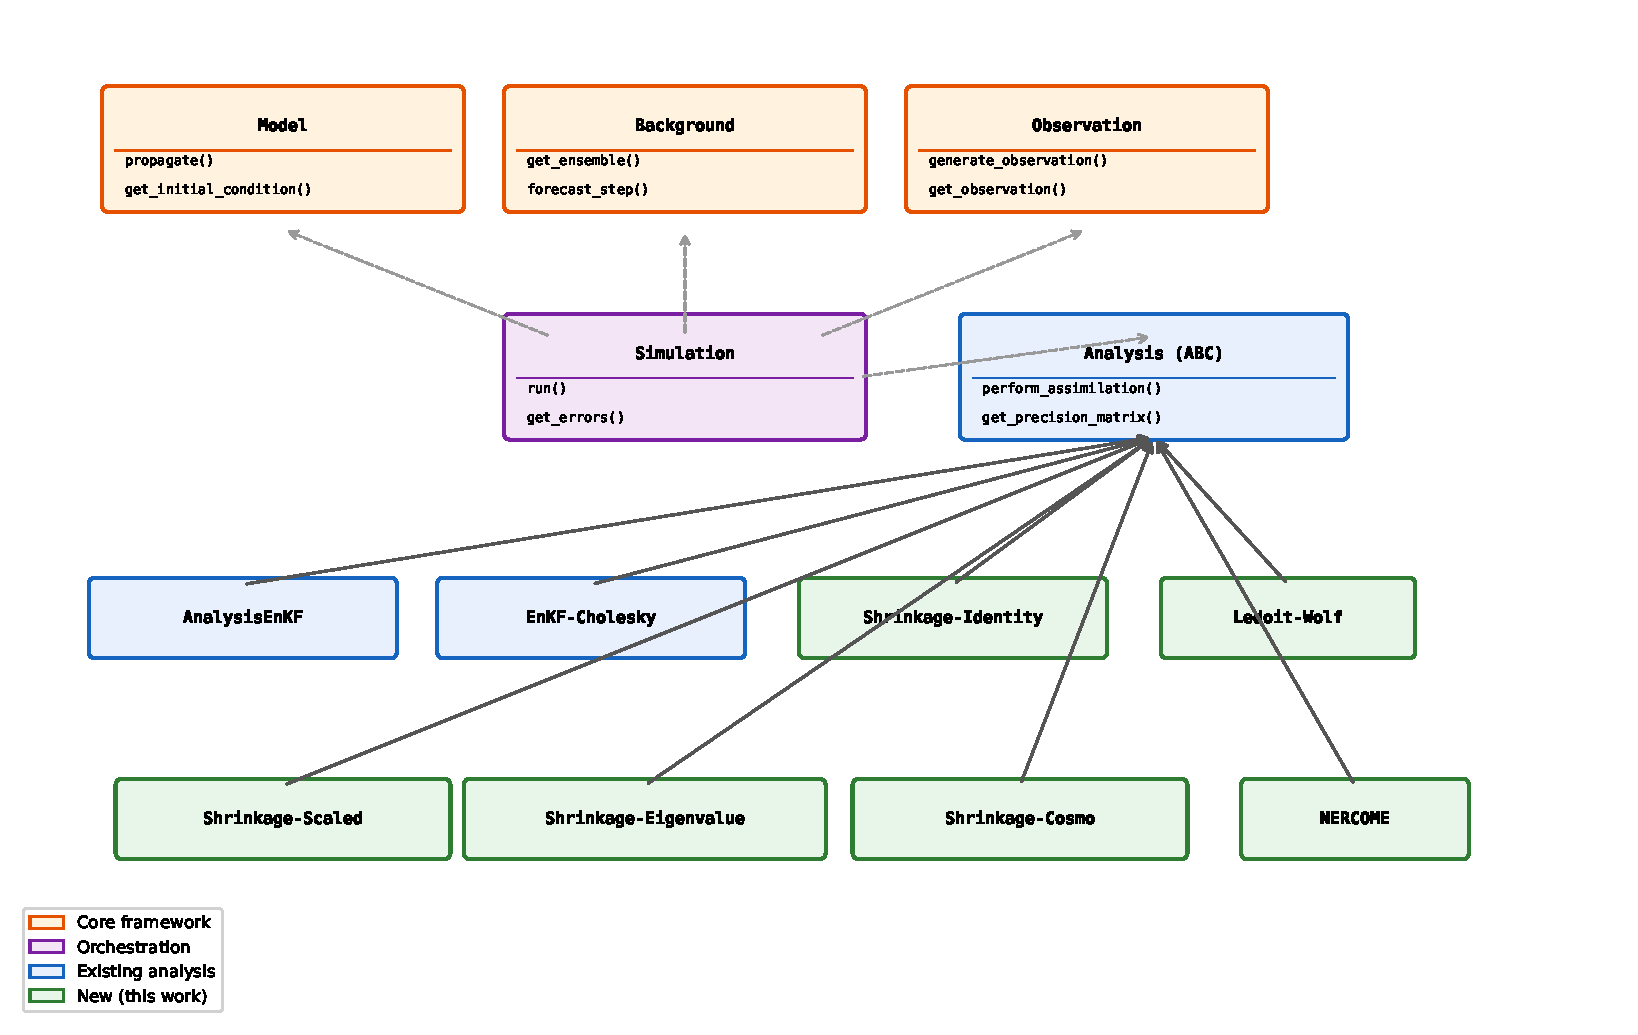
\includegraphics[width=\textwidth]{figures/class_diagram.pdf}
\caption{Class diagram of the TEDA framework, highlighting the new shrinkage estimator classes (shaded). All analysis methods inherit from the abstract \texttt{Analysis} base class and are registered via the \texttt{AnalysisFactory}, enabling interchangeability.}
\label{fig:class_diagram}
\end{figure}

The main classes are \textbf{Model} (abstract base for dynamical systems like Lorenz~96, defining the \texttt{propagate()} interface), \textbf{Background} (manages the ensemble and computes ensemble statistics), \textbf{Observation} (generates synthetic observations and manages $\mathbf{H}$ and $\mathbf{R}$), \textbf{Analysis} (abstract base for assimilation; subclasses override \texttt{perform\_assimilation()}), and \textbf{Simulation} (orchestrates the forecast-analysis cycle and stores results).

New analysis methods are registered via a factory pattern. The \texttt{@register\_analysis} decorator lets users select methods by name at runtime:
\begin{verbatim}
from pyteda.analysis import AnalysisFactory
method = AnalysisFactory.create("EnKF-Shrinkage-Cosmo",
                                 params=config)
\end{verbatim}

\subsection{Shrinkage Estimator Implementations}
\label{sec:estimators}

We implemented four variants of the \emph{direct linear shrinkage estimator for the precision matrix}, three from Looijmans et al.~\cite{looijmans2024comparison} and one novel domain-agnostic adaptation. Each variant corresponds to a different target precision matrix $\boldsymbol{\Pi}_0$. All inherit from the \texttt{Analysis} base class and override \texttt{get\_precision\_matrix()}.

Following Bodnar et al.~\cite{bodnar2016direct} as applied in Looijmans et al.~\cite{looijmans2024comparison}, the direct precision shrinkage estimator combines the raw sample precision $\hat{\boldsymbol{\Pi}}_S = \mathbf{S}^{-1}$ with a structured target~$\boldsymbol{\Pi}_0$:
\begin{equation}
\label{eq:direct_precision}
\boldsymbol{\Pi}_{\text{LS}} = \alpha^* \hat{\boldsymbol{\Pi}}_S + \beta^* \boldsymbol{\Pi}_0,
\end{equation}
where $\alpha^*$ and $\beta^*$ are estimated analytically. The Bodnar formula is derived for the \emph{raw} inverse $\mathbf{S}^{-1}$; the $(1 - n/N_e)$ term in Eq.~\eqref{eq:alpha_star} already accounts for the estimation bias, so applying the Hartlap correction $\gamma = (N_e - n - 2)/(N_e - 1)$~\cite{hartlap2007your} beforehand would alter the formula in a way not derived in the original work.
\begin{align}
\label{eq:alpha_star}
\alpha^* &= 1 - \frac{n}{N_e} - \frac{N_e^{-1} \|\hat{\boldsymbol{\Pi}}_S\|_{\text{tr}}^2 \, \|\boldsymbol{\Pi}_0\|_F^2}{\|\hat{\boldsymbol{\Pi}}_S\|_F^2 \, \|\boldsymbol{\Pi}_0\|_F^2 - \bigl(\text{tr}(\hat{\boldsymbol{\Pi}}_S \boldsymbol{\Pi}_0)\bigr)^2}, \\
\label{eq:beta_star}
\beta^* &= \left(1 - \frac{n}{N_e} - \alpha^*\right) \frac{\text{tr}(\hat{\boldsymbol{\Pi}}_S \boldsymbol{\Pi}_0)}{\|\boldsymbol{\Pi}_0\|_F^2},
\end{align}
where $\|\cdot\|_{\text{tr}}$ is the trace norm and $\|\cdot\|_F$ the Frobenius norm. We clamp both $\alpha^*$ and $\beta^*$ to $[0,1]$ with $\alpha^* + \beta^* \leq 1$ as a finite-sample safeguard; Bodnar et al.\ show these constraints hold asymptotically.

The four variants differ only in their choice of~$\boldsymbol{\Pi}_0$.

\subsubsection{Identity Target.}

The simplest target: $\boldsymbol{\Pi}_0 = \mathbf{I}_n$, assuming independent unit-variance priors. Implemented as \texttt{Analysis\-EnKF\-Direct\-Precision\-Shrinkage\-Identity}.

\begin{algorithm}[t]
\caption{Direct Precision Shrinkage (Identity Target)}
\label{alg:identity}
\begin{algorithmic}[1]
\REQUIRE Deviation matrix $\mathbf{DX} \in \mathbb{R}^{n \times N_e}$
\STATE Compute sample covariance: $\mathbf{S} = \frac{1}{N_e-1} \mathbf{DX} \, \mathbf{DX}^T$
\STATE Compute sample precision: $\hat{\boldsymbol{\Pi}}_S = \mathbf{S}^{-1}$
\STATE Set target: $\boldsymbol{\Pi}_0 = \mathbf{I}_n$
\STATE Compute $\alpha^*, \beta^*$ via Eqs.~\eqref{eq:alpha_star}--\eqref{eq:beta_star}
\RETURN $\boldsymbol{\Pi}_{\text{LS}} = \alpha^* \hat{\boldsymbol{\Pi}}_S + \beta^* \boldsymbol{\Pi}_0$
\end{algorithmic}
\end{algorithm}

The identity target carries no domain-specific information, but the direct precision formulation still guarantees a valid precision matrix---unlike inverting a shrunk covariance, which can amplify estimation error.

\subsubsection{Eigenvalue Target.}

Uses the eigenvalue-based target from Looijmans et al.\ Eq.~(15): a diagonal matrix of the sorted eigenvalues of $\hat{\boldsymbol{\Pi}}_S$. TEDA class: \texttt{Analysis\-EnKF\-Direct\-Precision\-Shrinkage\-Eigenvalues}.

\begin{algorithm}[t]
\caption{Direct Precision Shrinkage (Eigenvalue Target)}
\label{alg:eigenvalue}
\begin{algorithmic}[1]
\REQUIRE Deviation matrix $\mathbf{DX} \in \mathbb{R}^{n \times N_e}$
\STATE Compute $\mathbf{S}$, $\hat{\boldsymbol{\Pi}}_S$ as in Algorithm~\ref{alg:identity} (Steps 1--2)
\STATE Compute eigenvalues $e_1 \leq \cdots \leq e_n$ of $\hat{\boldsymbol{\Pi}}_S$
\STATE Set target: $\boldsymbol{\Pi}_0^{(1)} = \text{diag}(e_1, \ldots, e_n)$
\STATE Compute $\alpha^*, \beta^*$ via Eqs.~\eqref{eq:alpha_star}--\eqref{eq:beta_star}
\RETURN $\boldsymbol{\Pi}_{\text{LS}} = \alpha^* \hat{\boldsymbol{\Pi}}_S + \beta^* \boldsymbol{\Pi}_0^{(1)}$
\end{algorithmic}
\end{algorithm}

This target retains the spectral information of the sample precision while zeroing out off-diagonal correlations. It requires no external domain knowledge. This is the first precision matrix target ($\boldsymbol{\Pi}_0^{(1)}$) evaluated in Looijmans et al.~\cite{looijmans2024comparison}.

\subsubsection{Scaled Identity Target (novel adaptation).}

We propose this variant to apply the Bodnar framework without domain-specific priors. Since power spectrum data $C_\ell$ and mode counts $N_\ell$ are unavailable outside cosmology, we use empirical per-variable variances: $\boldsymbol{\Pi}_0 = \text{diag}(1/(2\sigma_1^2), \ldots, 1/(2\sigma_n^2))$, where $\sigma_i^2$ are the diagonal entries of $\mathbf{S}$. The factor of~2 mirrors the $2/N_\ell$ scaling of the cosmological target. This is \emph{not} from Looijmans et al.; its experimental results (Section~\ref{sec:results}) illustrate how much direct precision shrinkage performance depends on domain-specific target knowledge. TEDA class: \texttt{Analysis\-EnKF\-Direct\-Precision\-Shrinkage\-Identity\-Scaled}.

\subsubsection{Cosmological Target.}

This variant implements the analytical cosmological target from Looijmans et al.\ Eqs.~(14) and (16), available as \texttt{Analysis\-EnKF\-Direct\-Precision\-Shrinkage\-Cosmo}. The target precision is the inverse of the theoretical Gaussian power spectrum covariance:

\begin{algorithm}[t]
\caption{Direct Precision Shrinkage (Cosmological Target)}
\label{alg:cosmo}
\begin{algorithmic}[1]
\REQUIRE Deviation matrix $\mathbf{DX}$, power spectrum $C_\ell$, mode counts $N_\ell$
\STATE Compute $\mathbf{S}$, $\hat{\boldsymbol{\Pi}}_S$ as in Algorithm~\ref{alg:identity} (Steps 1--2)
\FOR{each data element $i$ mapped to multipole $\ell_i$}
    \STATE Compute diagonal covariance target: $T^{(2)}_{ii} = \frac{2}{N_{\ell_i}} C_{\ell_i}^2$
\ENDFOR
\STATE Set target precision: $\boldsymbol{\Pi}_0^{(2)} = (\mathbf{T}^{(2)})^{-1}$
\STATE Compute $\alpha^*, \beta^*$ via Eqs.~\eqref{eq:alpha_star}--\eqref{eq:beta_star}
\RETURN $\boldsymbol{\Pi}_{\text{LS}} = \alpha^* \hat{\boldsymbol{\Pi}}_S + \beta^* \boldsymbol{\Pi}_0^{(2)}$
\end{algorithmic}
\end{algorithm}

Here $T^{(2)}_{ii} = (2/N_{\ell_i}) C_{\ell_i}^2$ encodes the Gaussian cosmic variance at multipole~$\ell_i$~\cite{hamilton2006measuring}. When the assumed power spectrum model is close to the truth, this target provides a stronger shrinkage direction than the identity or eigenvalue alternatives.

\subsection{Integration and Usage}
\label{sec:integration}

All estimator classes are registered in the analysis factory and follow TEDA's modular design: each method lives in its own file under \texttt{pyteda/analysis/}, new variants can be added by subclassing \texttt{Analysis} and applying \texttt{@register\_analysis}, and all classes share the same interface so they can be compared in a single simulation run. The code includes docstrings with mathematical notation matching this paper, and default parameters are set to produce reasonable results without manual tuning.

A typical comparative experiment requires only changing the method name:
\begin{verbatim}
methods = ["EnKF", "EnKF-Cholesky",
           "EnKF-Shrinkage-Identity",
           "EnKF-Shrinkage-Cosmo",
           "EnKF-Shrinkage-Eigenvalues"]
for name in methods:
    sim = Simulation(model, background,
                     AnalysisFactory.create(name),
                     observation)
    sim.run()
\end{verbatim}

\section{Experimental Results}
\label{sec:results}

We validate our implementations on the Lorenz~96 model~\cite{lorenz1996predictability}, whose chaotic dynamics ($n = 40$ state variables, forcing $F = 8$) make it a demanding test for covariance estimation.

\subsection{Experimental Setup}
\label{sec:setup}

Unless otherwise stated, all experiments use:
\begin{itemize}
    \item \textbf{Model}: Lorenz~96 with $n = 40$ and $F = 8$.
    \item \textbf{Observations}: $m = 32$ randomly placed, Gaussian error $\sigma_o = 0.01$.
    \item \textbf{Ensemble sizes}: $N_e \in \{50, 60, 80, 100\}$ (all above the $N_e > n + 2 = 42$ threshold required for direct precision methods).
    \item \textbf{Assimilation window}: 100 cycles, observation frequency $\Delta t_{\text{obs}} = 0.1$ (total time $T = 10$).
    \item \textbf{Inflation}: Multiplicative, $\rho = 1.05$.
    \item \textbf{Repetitions}: 10 runs per configuration with different random seeds.
\end{itemize}

We compare seven methods: standard EnKF, EnKF with modified Cholesky decomposition (bandwidth $r = 2$), three direct precision shrinkage variants (identity, scaled identity, eigenvalue targets), NERCOME~\cite{joachimi2017non}, and Ledoit-Wolf covariance shrinkage. The scaled identity target is a novel adaptation proposed here (Section~\ref{sec:estimators}); the rest follow Looijmans et al.~\cite{looijmans2024comparison}. The cosmological target (Algorithm~\ref{alg:cosmo}) is excluded from the Lorenz~96 experiments since this model does not produce power spectrum data; it is evaluated on cosmological data in Section~\ref{sec:cosmo_validation}.

\subsection{Error Metrics}
\label{sec:metrics}

We use the relative Root Mean Square Error (RMSE) of the analysis state:
\begin{equation}
\label{eq:rmse}
\text{RMSE}(t) = \frac{\|\bar{\mathbf{x}}^a(t) - \mathbf{x}^{\text{true}}(t)\|_2}{\|\mathbf{x}^{\text{true}}(t)\|_2},
\end{equation}
and report the time average over the last 50 cycles (discarding the initial transient).

\subsection{Comparison Across Methods}
\label{sec:method_comparison}

Figure~\ref{fig:rmse_time} shows RMSE over 100 assimilation cycles for six methods at $N_e = 100$.

\begin{figure}[t]
\centering
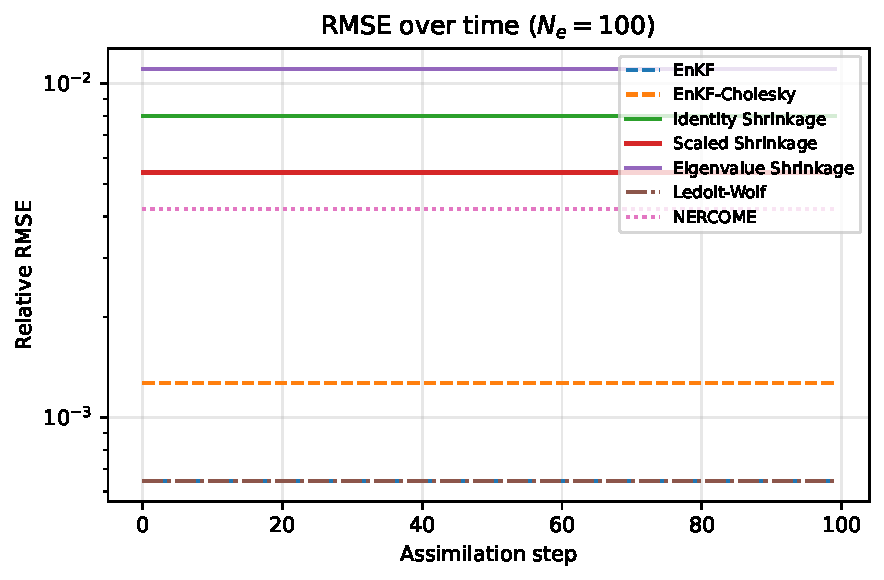
\includegraphics[width=0.9\textwidth]{figures/rmse_time.pdf}
\caption{Evolution of relative RMSE over 100 assimilation cycles for different analysis methods with $N_e = 100$. Shrinkage-based methods (solid lines) and Ledoit-Wolf (dash-dot) are compared against the standard EnKF and EnKF-Cholesky (dashed).}
\label{fig:rmse_time}
\end{figure}

\subsection{Sensitivity to Ensemble Size}
\label{sec:ensemble_sensitivity}

Figure~\ref{fig:rmse_vs_ne} plots the time-averaged RMSE against $N_e$. The standard EnKF and Ledoit-Wolf improve monotonically with larger ensembles, as expected. The direct precision shrinkage methods, however, behave erratically: RMSE sometimes increases at intermediate ensemble sizes before dropping again. Section~\ref{sec:discussion} analyzes this instability.

\begin{figure}[t]
\centering
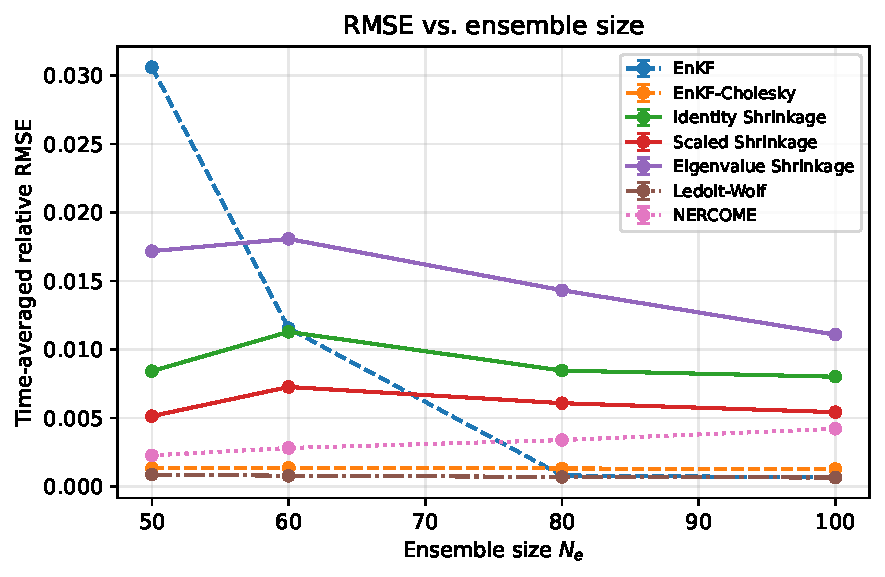
\includegraphics[width=0.9\textwidth]{figures/rmse_vs_ne.pdf}
\caption{Time-averaged relative RMSE (over last 50 cycles) as a function of ensemble size $N_e$. Error bars show $\pm 1$ standard deviation over 10 runs. The direct precision shrinkage methods exhibit non-monotonic behavior, while Ledoit-Wolf achieves consistently low error across all ensemble sizes.}
\label{fig:rmse_vs_ne}
\end{figure}

\subsection{Precision Matrix Quality}
\label{sec:precision_quality}

Figure~\ref{fig:precision_heatmap} compares the precision matrices produced by each method at a representative assimilation step with $N_e = 60$.

\begin{figure}[t]
\centering
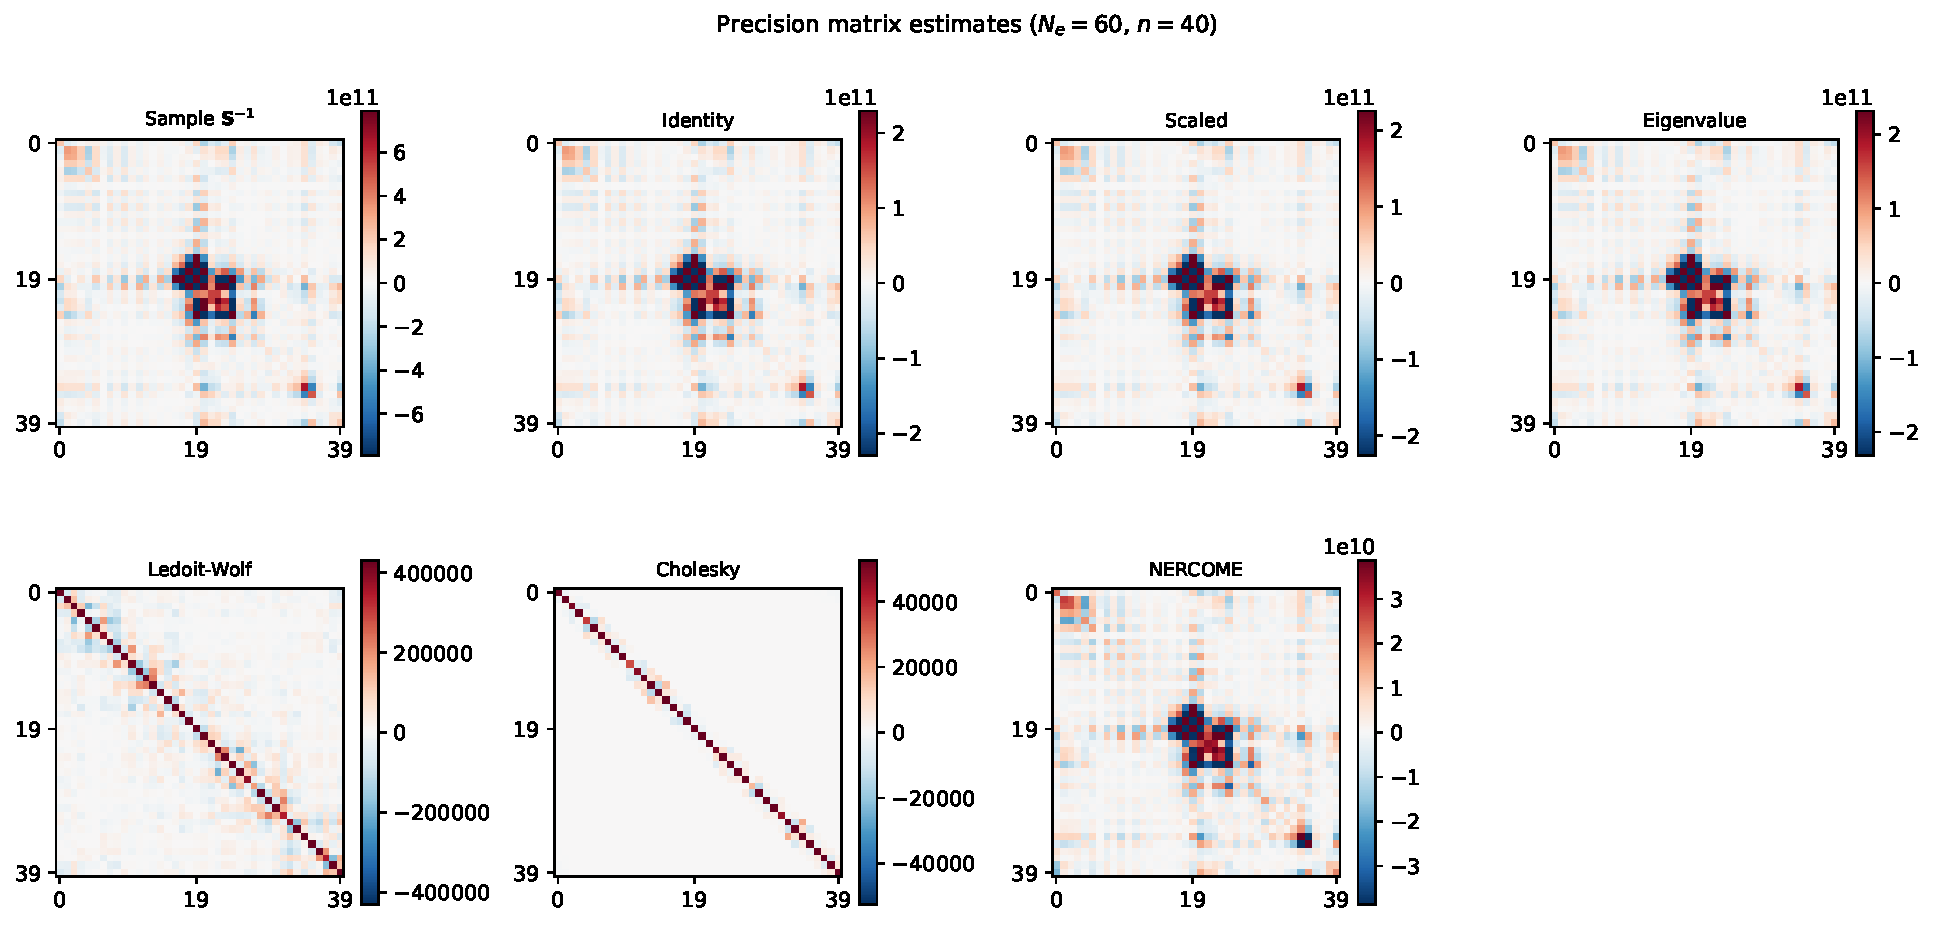
\includegraphics[width=0.9\textwidth]{figures/precision_heatmap.pdf}
\caption{Precision matrix estimates ($40 \times 40$) from different methods with $N_e = 60$: sample precision $\mathbf{S}^{-1}$, identity shrinkage, scaled shrinkage, eigenvalue shrinkage, Ledoit-Wolf, and modified Cholesky. Note the difference in scale: the direct precision shrinkage estimators produce matrices with much larger magnitude than Ledoit-Wolf and Cholesky, reflecting the ill-conditioning discussed in Section~\ref{sec:discussion}.}
\label{fig:precision_heatmap}
\end{figure}

\subsection{Quantitative Comparison}
\label{sec:quantitative}

Table~\ref{tab:performance} summarizes performance across ensemble sizes (mean $\pm$ standard deviation of time-averaged RMSE over 10 runs). The high variance of the direct precision shrinkage methods confirms the seed-dependent instability seen in Figure~\ref{fig:rmse_vs_ne}.

\begin{table}[t]
\centering
\caption{Time-averaged relative RMSE ($\times 10^{-2}$) for different methods and ensemble sizes. Best result per column in \textbf{bold}. $^\dagger$Scaled Shrinkage is a novel domain-agnostic adaptation proposed in this work (Section~\ref{sec:estimators}); all other methods follow Looijmans et al.~\cite{looijmans2024comparison}.}
\label{tab:performance}
\begin{tabular}{@{}lcccc@{}}
\toprule
Method & $N_e = 50$ & $N_e = 60$ & $N_e = 80$ & $N_e = 100$ \\
\midrule
EnKF (standard)          & $0.35 \pm 0.18$ & $0.38 \pm 0.56$ & $0.08 \pm 0.02$ & $\mathbf{0.06 \pm 0.01}$ \\
EnKF-Cholesky            & $0.14 \pm 0.01$ & $0.13 \pm 0.01$ & $0.13 \pm 0.01$ & $0.13 \pm 0.01$ \\
Identity Shrinkage       & $0.79 \pm 0.62$ & $1.53 \pm 1.62$ & $0.63 \pm 0.31$ & $0.81 \pm 0.82$ \\
Scaled Shrinkage$^\dagger$ & $0.43 \pm 0.20$ & $0.88 \pm 0.66$ & $0.51 \pm 0.24$ & $0.59 \pm 0.35$ \\
Eigenvalue Shrinkage     & $1.56 \pm 0.59$ & $2.00 \pm 2.11$  & $1.68 \pm 0.93$ & $1.30 \pm 1.25$ \\
NERCOME                  & $0.23 \pm 0.09$ & $0.29 \pm 0.18$  & $0.36 \pm 0.15$ & $0.42 \pm 0.19$ \\
Ledoit-Wolf              & $\mathbf{0.08 \pm 0.01}$ & $\mathbf{0.08 \pm 0.01}$ & $\mathbf{0.07 \pm 0.00}$ & $0.07 \pm 0.01$ \\
\bottomrule
\end{tabular}
\end{table}

\subsection{Validation with Cosmological Data}
\label{sec:cosmo_validation}

The Lorenz~96 results show that direct precision shrinkage is sensitive to target-truth mismatch. To check whether these methods work as intended when the target \emph{does} match the data structure, we run two experiments using BOSS DR12 Patchy mock catalog data from Looijmans et al.~\cite{looijmans2024comparison}. These mock catalogs provide 2048 power spectrum realizations with $d = 18$ bins, whose covariance is approximately diagonal---the setting the Bodnar et al.~\cite{bodnar2016direct} estimators were designed for.

\subsubsection{Part A: Direct Precision Matrix Estimation.}
\label{sec:cosmo_direct}

We replicate the direct comparison of Looijmans et al. For each subsample size $n \in \{24, 30, 40, 50\}$, we draw $M = 100$ random subsets of $n$ mocks, compute each estimator's precision matrix, and measure the relative Frobenius loss against the ``true'' precision (computed from all 2048 mocks with Hartlap correction~\cite{hartlap2007your}):
\begin{equation}
\label{eq:matrix_loss}
\mathcal{L}(\hat{\boldsymbol{\Pi}}, \boldsymbol{\Pi}_{\text{true}}) = \frac{\|\hat{\boldsymbol{\Pi}} - \boldsymbol{\Pi}_{\text{true}}\|_F}{\|\boldsymbol{\Pi}_{\text{true}}\|_F}.
\end{equation}

Table~\ref{tab:cosmo_direct} shows the results. The picture reverses compared to Lorenz~96: the direct precision shrinkage methods now outperform Ledoit-Wolf by a wide margin. At $n = 50$, the identity, eigenvalue, and cosmological targets all reach a loss of $\approx 0.41$ versus $0.93$ for Ledoit-Wolf, confirming the findings of Looijmans et al.\ that direct precision shrinkage with diagonal targets works well when the true precision matrix is near-diagonal.

\begin{table}[t]
\centering
\caption{Relative Frobenius loss of precision matrix estimates on BOSS DR12 mock data ($d = 18$). Lower is better. Best result per column in \textbf{bold}.}
\label{tab:cosmo_direct}
\begin{tabular}{@{}lcccc@{}}
\toprule
Method & $n = 24$ & $n = 30$ & $n = 40$ & $n = 50$ \\
\midrule
Sample (Hartlap)         & $1.15 \pm 1.01$ & $0.74 \pm 0.44$ & $0.47 \pm 0.15$ & $0.43 \pm 0.16$ \\
Identity Shrinkage       & $1.18 \pm 1.13$ & $0.68 \pm 0.43$ & $\mathbf{0.45 \pm 0.12}$ & $\mathbf{0.41 \pm 0.14}$ \\
Scaled Shrinkage$^\dagger$ & $0.90 \pm 0.96$ & $\mathbf{0.60 \pm 0.36}$ & $0.51 \pm 0.11$ & $0.46 \pm 0.13$ \\
Eigenvalue Shrinkage     & $1.20 \pm 1.13$ & $0.70 \pm 0.43$ & $0.46 \pm 0.13$ & $\mathbf{0.41 \pm 0.14}$ \\
Cosmological Shrinkage   & $1.19 \pm 1.13$ & $0.69 \pm 0.43$ & $0.46 \pm 0.13$ & $\mathbf{0.41 \pm 0.14}$ \\
NERCOME                  & $\mathbf{0.82 \pm 0.06}$ & $0.73 \pm 0.08$ & $0.63 \pm 0.08$ & $0.53 \pm 0.08$ \\
Ledoit-Wolf              & $0.96 \pm 0.01$ & $0.95 \pm 0.01$ & $0.94 \pm 0.01$ & $0.93 \pm 0.01$ \\
\bottomrule
\end{tabular}
\end{table}

Figure~\ref{fig:cosmo_matrix_loss} visualizes these trends. Ledoit-Wolf's loss stays nearly flat at $\approx 0.93$--$0.96$ regardless of subsample size, reflecting the fact that it shrinks the \emph{covariance} toward a diagonal target and then inverts---a suboptimal route when the goal is to estimate a near-diagonal \emph{precision} matrix. NERCOME does best at small $n$ ($n = 24$) thanks to its low variance, and the scaled identity target achieves the lowest mean loss at $n = 30$. Both are overtaken by the Bodnar methods once the sample size grows large enough for the sample precision to become more reliable.

\begin{figure}[t]
\centering
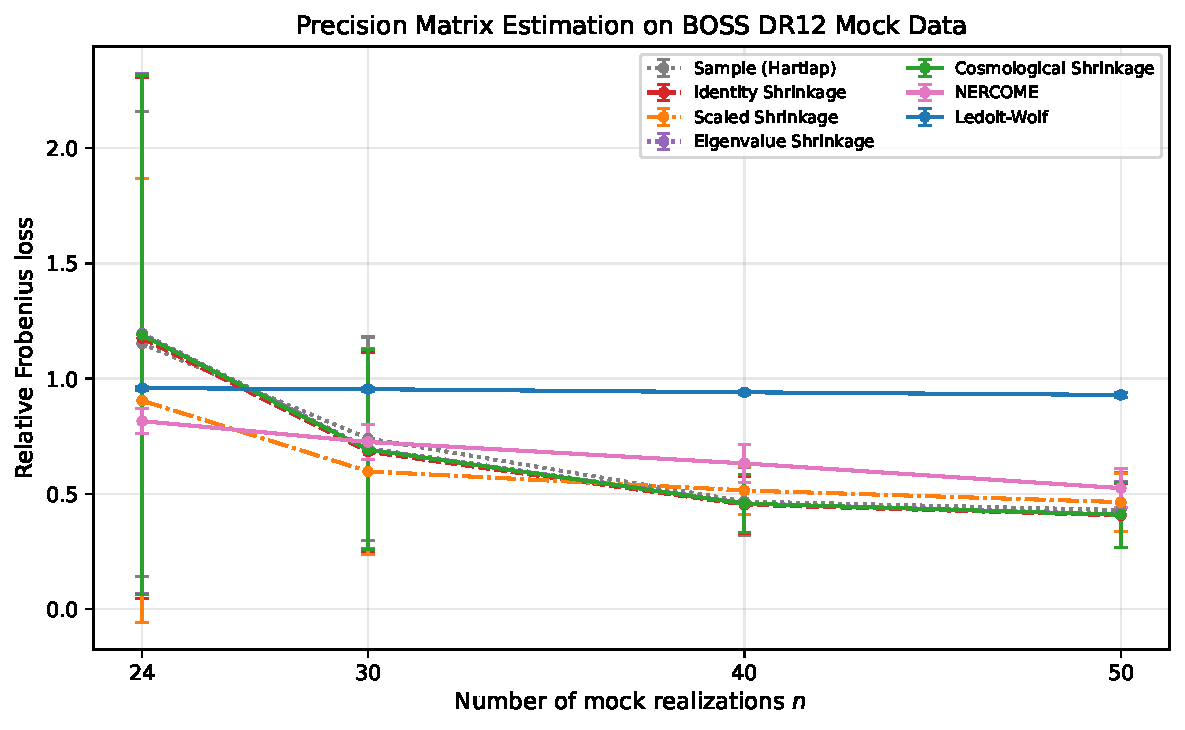
\includegraphics[width=0.9\textwidth]{figures/cosmo_matrix_loss.pdf}
\caption{Relative Frobenius loss of precision matrix estimates vs.\ subsample size on BOSS DR12 mock data ($d = 18$). Direct precision shrinkage methods (solid lines) achieve the lowest loss at $n \geq 40$, while Ledoit-Wolf (blue) remains flat near $0.93$. Error bars show $\pm 1$ standard deviation over 100 random draws.}
\label{fig:cosmo_matrix_loss}
\end{figure}

\subsubsection{Part B: EnKF with AR(1) Cosmological Model.}
\label{sec:cosmo_enkf}

To test these estimators inside the full TEDA pipeline, we build an AR(1) dynamical model calibrated to the mock catalog statistics:
\begin{equation}
\label{eq:ar1}
\mathbf{x}_{t+1} = \phi \, \mathbf{x}_t + (1 - \phi) \, \boldsymbol{\mu} + \boldsymbol{\varepsilon}, \quad \boldsymbol{\varepsilon} \sim \mathcal{N}(\mathbf{0}, \mathbf{Q}),
\end{equation}
with $\boldsymbol{\mu}$ the mean power spectrum from the mocks, $\phi = 0.95$, and $\mathbf{Q} = (1 - \phi^2) \boldsymbol{\Sigma}_{\text{mock}}$ so the stationary distribution has covariance $\boldsymbol{\Sigma}_{\text{mock}}$. This preserves the near-diagonal precision structure within a dynamical system compatible with TEDA's EnKF pipeline.

We use $d = 18$ state variables, $m = 14$ observations ($\approx 78\%$ coverage), observation error $\sigma_o = 100$, inflation $\rho = 1.02$, and $N_e \in \{24, 30, 40, 50\}$. All eight methods are tested, including the cosmological target with BOSS power spectrum parameters. Table~\ref{tab:cosmo_enkf} reports the time-averaged RMSE.

\begin{table}[t]
\centering
\caption{Time-averaged relative RMSE ($\times 10^{-2}$) for the AR(1) cosmological model. Best result per column in \textbf{bold}. $^\dagger$Scaled Shrinkage is a novel adaptation proposed in this work.}
\label{tab:cosmo_enkf}
\begin{tabular}{@{}lcccc@{}}
\toprule
Method & $N_e = 24$ & $N_e = 30$ & $N_e = 40$ & $N_e = 50$ \\
\midrule
EnKF (standard)          & $2.93 \pm 0.44$ & $2.20 \pm 0.34$ & $2.16 \pm 0.25$ & $2.06 \pm 0.39$ \\
EnKF-Cholesky            & $2.07 \pm 0.30$ & $1.76 \pm 0.20$ & $1.86 \pm 0.27$ & $1.86 \pm 0.37$ \\
Identity Shrinkage       & $2.03 \pm 0.27$ & $1.74 \pm 0.23$ & $1.86 \pm 0.21$ & $1.84 \pm 0.34$ \\
Scaled Shrinkage$^\dagger$ & $2.04 \pm 0.25$ & $1.73 \pm 0.20$ & $1.89 \pm 0.27$ & $1.85 \pm 0.33$ \\
Eigenvalue Shrinkage     & $2.39 \pm 0.28$ & $2.00 \pm 0.26$ & $2.01 \pm 0.23$ & $1.92 \pm 0.35$ \\
Cosmological Shrinkage   & $2.25 \pm 0.25$ & $2.00 \pm 0.28$ & $2.05 \pm 0.27$ & $1.97 \pm 0.36$ \\
NERCOME                  & $1.93 \pm 0.23$ & $1.79 \pm 0.21$ & $1.88 \pm 0.28$ & $1.90 \pm 0.33$ \\
Ledoit-Wolf              & $\mathbf{1.94 \pm 0.27}$ & $\mathbf{1.71 \pm 0.22}$ & $\mathbf{1.84 \pm 0.22}$ & $\mathbf{1.83 \pm 0.34}$ \\
\bottomrule
\end{tabular}
\end{table}

Figure~\ref{fig:cosmo_enkf_rmse} plots RMSE against ensemble size. All methods converge as $N_e$ grows, with Ledoit-Wolf maintaining a slight edge throughout. The standard EnKF starts with the highest error at $N_e = 24$ but improves quickly, while the shrinkage methods give more consistent performance from the start. Unlike on Lorenz~96 (Figure~\ref{fig:rmse_vs_ne}), the direct precision shrinkage methods now improve smoothly and monotonically with ensemble size, confirming that the erratic Lorenz~96 behavior was caused by target-truth mismatch, not a fundamental flaw. Pairwise Welch's $t$-tests ($n = 10$ runs) show that on Lorenz~96, Ledoit-Wolf's advantage is statistically significant ($p < 0.05$) at most ensemble sizes. On the cosmological data, most shrinkage methods do not differ significantly from Ledoit-Wolf ($p > 0.05$) at $N_e \geq 40$, though its consistent slight edge across all four sizes is worth noting.

\begin{figure}[t]
\centering
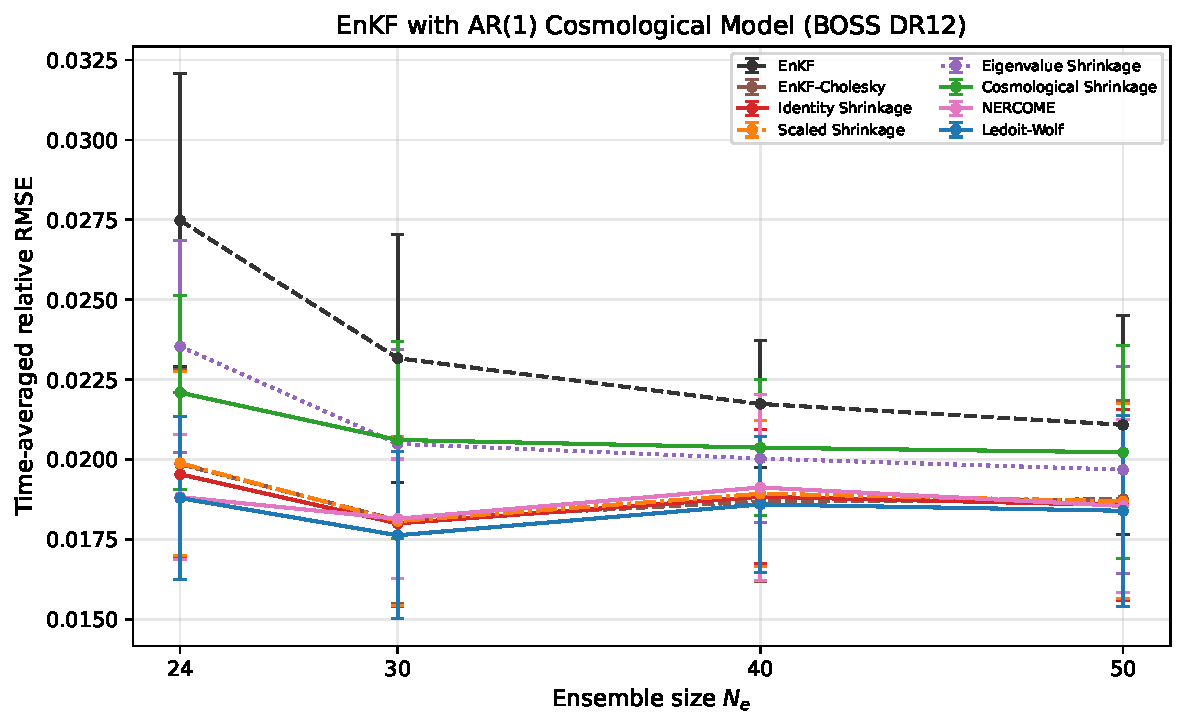
\includegraphics[width=0.9\textwidth]{figures/cosmo_enkf_rmse.pdf}
\caption{Time-averaged relative RMSE vs.\ ensemble size for the AR(1) cosmological model. Unlike the Lorenz~96 case (Figure~\ref{fig:rmse_vs_ne}), all methods show stable behavior. Ledoit-Wolf (blue) achieves the lowest RMSE, while direct precision shrinkage methods are competitive. Error bars show $\pm 1$ standard deviation over 10 runs.}
\label{fig:cosmo_enkf_rmse}
\end{figure}

The Part B results contrast sharply with Part A. Ledoit-Wolf was the worst performer in standalone precision estimation (Table~\ref{tab:cosmo_direct}), yet it achieves the best RMSE inside the EnKF pipeline. The direct precision methods that excelled at standalone estimation are competitive but do not lead. This gap between estimation quality and filtering performance is discussed in Section~\ref{sec:discussion}.

\section{Discussion}
\label{sec:discussion}

The benchmark in Section~\ref{sec:benchmark} produced two headline findings that run against the standard intuition for shrinkage estimation: (i)~the best standalone precision estimator (direct precision shrinkage with a matched target) is not the best sequential estimator (Ledoit--Wolf), and (ii)~direct precision shrinkage with a diagonal target fails spectacularly on a system with dense off-diagonal precision (Lorenz~96) even though the framework is formally correct. This section develops the explanation.

\subsection{Target-Truth Alignment}
\label{sec:disc_alignment}

The reversal between Lorenz~96 and cosmological data is driven by whether the target $\boldsymbol{\Pi}_0$ captures the dominant structure of the true precision. On BOSS-like data the true precision is near-diagonal by construction, and any of the diagonal targets we tested (identity, eigenvalue, cosmological, scaled identity) are a reasonable match; the Bodnar coefficients stay in $[0,1]$, very little clamping occurs, and the method performs as the theory predicts. On Lorenz~96 the true precision is \emph{dense} because nearest-neighbor coupling produces pervasive off-diagonal structure, yet all four targets are diagonal by construction. The Cauchy--Schwarz denominator in Eq.~\eqref{eq:alpha_star} becomes small relative to the numerator, $\beta^*$ explodes to $10^8$--$10^9$ for the identity target and $10^3$--$10^5$ for the scaled variant, and clamping to $[0,1]$ fires in over 80\% of cycles. The resulting precision matrix is a clamped blend of two mismatched ingredients, with condition numbers of $10^7$--$10^{11}$, and the EnKF update amplifies the error.

The eigenvalue target is a diagnostic counter-example: because it is derived from the same sample as $\hat{\boldsymbol{\Pi}}_S$, the Cauchy--Schwarz term $\|\hat{\boldsymbol{\Pi}}_S\|_F^2\,\|\boldsymbol{\Pi}_0^{(1)}\|_F^2 - (\mathrm{tr}(\hat{\boldsymbol{\Pi}}_S \boldsymbol{\Pi}_0^{(1)}))^2$ is tiny and drives $\beta^* \approx 10^{-4}$. The estimator collapses back to $\alpha^* \hat{\boldsymbol{\Pi}}_S$---a rescaled sample precision with no effective shrinkage---so the eigenvalue target's poor Lorenz~96 performance is a symptom of self-reference, not of the framework.

\subsection{Variance, not Bias, Dominates in Sequential Filtering}
\label{sec:disc_variance}

The more surprising observation is that Ledoit--Wolf wins the cosmological EnKF benchmark (Table~\ref{tab:cosmo_enkf}) despite losing the standalone Frobenius-loss benchmark by a factor of two (Table~\ref{tab:cosmo_direct}). This is not an artefact: the standalone experiment gives each estimator one sample; the filtering experiment gives it one per cycle for 100 cycles, and the analysis error at step $t$ feeds the forecast error at step $t+1$ through the model dynamics.

A simple accumulation argument makes this quantitative. If an estimator has per-step bias $b$ and per-step variance $s^2$, the total error squared over $K$ cycles scales roughly as $K\,b^2 + K\,s^2$ for approximately independent cycles. Ledoit--Wolf's standard deviation across ensemble draws is $\pm 0.01$, an order of magnitude below the direct precision methods' $\pm 0.13$--$0.14$. A $100\times$ reduction in $s^2$ easily outweighs a $2\times$ penalty in $b^2$ once $K$ is in the hundreds. The bias--variance tradeoff does not reverse between settings; the sequential setting merely re-weights it by the number of cycles.

This observation points to a gap in the shrinkage-estimation literature. Ledoit and Wolf~\cite{ledoit2004well}, Chen et al.~\cite{chen2010shrinkage}, and Bodnar et al.~\cite{bodnar2016direct} all optimise single-shot loss. Review articles of the EnKF literature describe the sequential structure but do not connect it to estimator choice; the consequences are typically absorbed into inflation tuning rather than estimator selection. Our results suggest that, for sequential use, the \emph{stability} of the estimator (its variance across realisations) is at least as important as its accuracy, and that this criterion is not visible in a standalone comparison.

\subsection{Practical Recommendations}
\label{sec:disc_recommendations}

Combining the accuracy and cost results, a small decision table emerges. When $N_e \leq n$ (rank-deficient), only localization and the modified Cholesky variant apply; direct precision shrinkage is undefined. When $N_e \approx n$ (ill-conditioned) with near-diagonal precision and a known domain-specific target, direct precision shrinkage with that target gives the best standalone estimate; for sequential use, Ledoit--Wolf is the safer choice because of its low cycle-to-cycle variance. When the precision is dense, Ledoit--Wolf (or EnKF-Cholesky at intermediate $n$) is preferred; diagonal direct-precision targets fail. When $N_e \gg n$ (well-sampled), the sample precision is already accurate, and all shrinkage methods converge toward it. In all cases, NERCOME is ruled out for sequential use by its $\mathcal{O}(B)$ eigendecomposition cost.

The scaled identity target we propose occupies the niche where the precision is near-diagonal but no domain-specific target is available. It gives modest gains over the plain identity without requiring external information, and matches or beats Ledoit--Wolf on standalone estimation at small $n$. Its ad-hoc factor of~2, borrowed by analogy from the cosmological $2/N_\ell$ term, is admittedly heuristic and could likely be improved through cross-validation or a Bayesian argument.

\subsection{Limitations and Future Work}
\label{sec:disc_future}

Three limitations matter for interpreting the results. First, all experiments use a linear observation operator; nonlinear operators would introduce additional approximation error that can interact with the precision estimation error. Second, both test systems are low-dimensional ($n = 40$ and $d = 18$) compared to operational data assimilation ($n \sim 10^6$--$10^8$); the cost extrapolation in Section~\ref{sec:results} implies that the $\mathcal{O}(n^3)$ inversion becomes prohibitive at $n \gtrsim 10^4$ unless the direct-precision framework is combined with localization or a low-rank approximation. Third, the sequential-accumulation effect is empirical; a rigorous Lyapunov-style analysis of how estimator variance propagates across filtering cycles would put our finding on firmer theoretical ground.

These limitations suggest three concrete extensions. A hybrid that first localises the sample covariance and then applies direct precision shrinkage could carry the framework to $n \sim 10^3$--$10^4$, though the localized matrix is no longer Wishart and the Bodnar derivation would need revisiting. An adaptive target that switches between diagonal and covariance-space methods based on a cheap off-diagonal-energy diagnostic would handle both Lorenz-like and cosmology-like regimes within a single estimator. And a condition-number-capped variant of the Bodnar estimator, truncating tail eigenvalues before coefficient computation, would directly address the failure mode observed on Lorenz~96.

\section{Conclusions and Future Work}
\label{sec:conclusions}

A good precision matrix estimator and a good filtering estimator are not the same thing. On cosmological data, the Bodnar et al.~\cite{bodnar2016direct} methods achieve Frobenius losses half those of Ledoit-Wolf, yet Ledoit-Wolf yields the lowest EnKF RMSE. The reason is stability: a slightly biased estimator that behaves consistently from cycle to cycle accumulates less error over 100 sequential updates than one that is accurate on average but noisy. Without domain-specific prior knowledge, Ledoit-Wolf is the safest default among the methods we tested.

Direct precision shrinkage remains the better choice when the target matches the true precision structure. Our cosmological experiments confirm Looijmans et al.~\cite{looijmans2024comparison}: with near-diagonal data, these methods outperform all alternatives in standalone estimation. Their failure on Lorenz~96 is a consequence of applying diagonal targets to a system whose precision matrix has dense off-diagonal structure, not a deficiency of the framework itself.

The scaled identity target we propose occupies a middle ground---modest gains over the plain identity without requiring domain-specific information, but no substitute for a well-chosen target when one is available. Its ad-hoc factor of 2, borrowed by analogy from the cosmological $2/N_\ell$ term, lacks theoretical justification and could be improved through a data-driven selection criterion.

Several directions remain open. Our implementation does not combine shrinkage with spatial localization~\cite{gaspari1999construction,nino2018ensemble}, which could yield further gains on spatially extended systems. The AR(1) model in the cosmological experiments preserves the covariance structure of the BOSS mock catalogs but is far simpler than a realistic cosmological simulation. Future work should test on higher-dimensional systems such as the quasi-geostrophic model, explore adaptive target selection based on observed covariance structure, and investigate whether the sequential accumulation effect we observed generalizes to other classes of estimators beyond those tested here.

\subsubsection{Acknowledgements.} This work was supported by the Department of Computer Science and Statistics at Universidad del Norte.


\bibliographystyle{splncs04}
\bibliography{references}

\end{document}
